The agent was trained on the training dataset and evaluated on the test dataset at patient-level. The performance of the resulting predictions for the SMS subscores and their summed SMS on the test dataset in terms of the $R^2$ are as shown in Table \ref{tab:ltfmresults}. This performance is comparable to the agreement of each expert recommendation with the collective decisions of the medical-board (see Figure \ref{fig:LTFMvsBoard}). For each evaluation of the test data, the agent was able to optimally select a feature set and a PM for a given stride-pair, yielding excellent predictive performance and delivering patient-specific key features, which could help medical experts identify personalized key therapeutic targets.
\begin{table}[H]
  \caption{Performance of RL agents on the test dataset in terms of $R^2$, and corresponding ICC\textsubscript{1.1} of the medical-board assessments.}
  \label{tab:ltfmresults}
  \begin{tabular}{|l|l|l|l|}
    \hline
    \textbf{SMS} & \textbf{Feature subset} & \textbf{$R^2$} & \textbf{ICC\textsubscript{1.1}} \\
    \textbf{subscore} & $|\fsubset|$ & & \\
    \hline
    Trunk-SMS     & 241 of 680 features & 0.59 $\,$ & 0.65 \\
    Leg-SMS       & 188 of 356 pre-selected features & 0.56 $\,$ & 0.73 \\
    Arm-SMS       & 99 of 330 pre-selected features & 0.54 $\,$ & 0.72 \\
    Speed-SMS     & 31 of 32 pre-selected features & 0.78 $\,$  & 0.72 \\
    Fluency-SMS   & 263 of 680 features & 0.73 $\,$ & 0.72 \\
    Stability-SMS & 238 of 680 features & 0.82 $\,$ & 0.83 \\
    \hline
    \multicolumn{2}{|l|}{Combination of subscore models to predict the SMS} & 0.83 & 0.88 \\
    \hline
  \end{tabular}
\end{table}
\begin{figure}[!h]
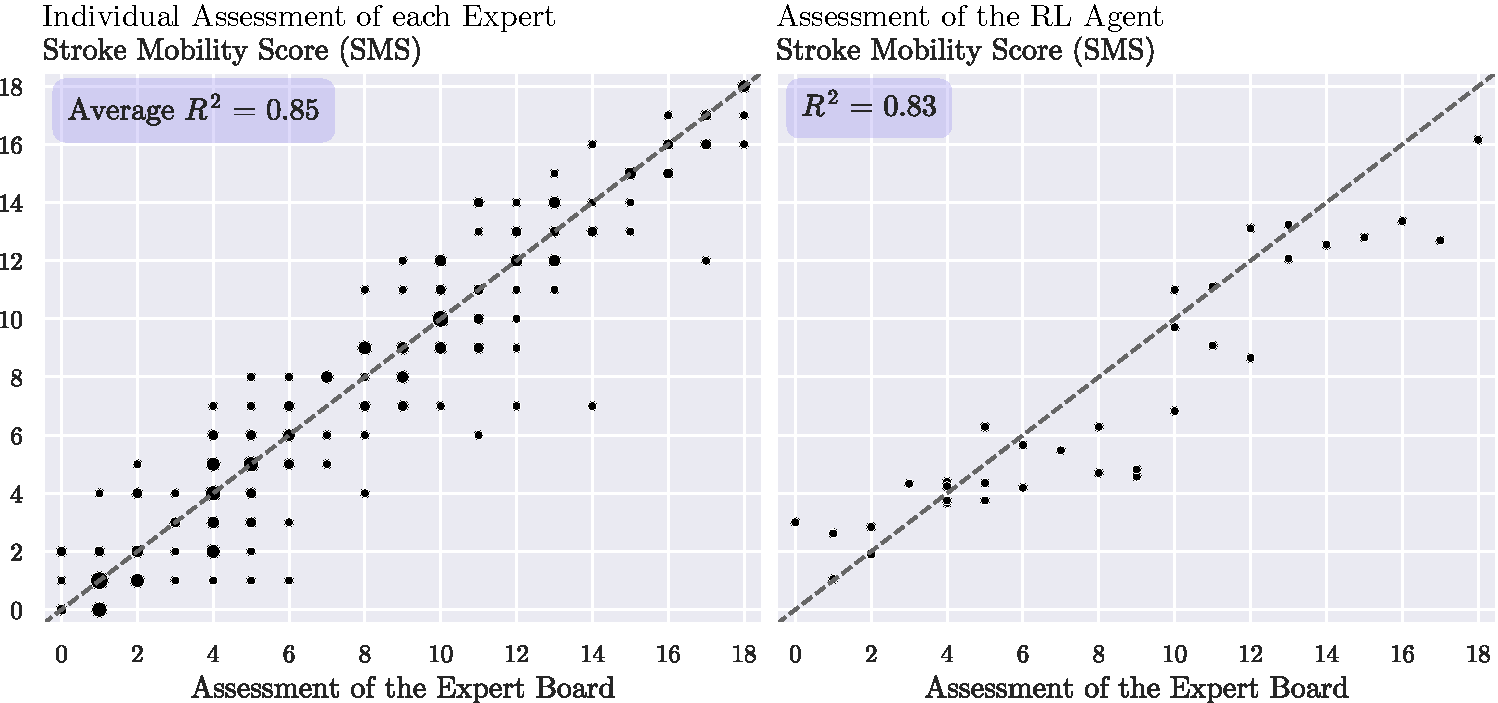
\includegraphics[width=\textwidth]{DoctorsvsBoard_TestSplit_and_LTFMJRMCC.pdf}
\caption{Scatterplots showing how the individual experts (left) and RL agent (right) compare with the medical-board's gait assessment (abscissa) in terms of the SMS.} \label{fig:LTFMvsBoard}
\end{figure}
To obtain a general overview of the salient features for the varying degrees of gait impairment, inference is performed on the training dataset, and the frequency of recruited features summed per SMS subscore. The intuititon here is that patients assigned the same SMS subscore should exhibit similar underlying physical characteristics, represented by a subset of key features. Upon observing a patient, a well-trained agent then recruits the features that make up the underlying pattern learned from patients of similar physical status. Consequently, the recruitment frequency of a feature can serve as an indication of the feature's representativeness with respect to a given SMS subscore group. Taking Fluency-SMS as an example, the top seven features and progression of the averaged $Q$-values per sampled batch during training are as shown in Table \ref{tab:featuresRecruitmentFrequency} and Figure \ref{fig:QValuesProgression}, respectively.
\begin{table}[H]
  \caption{Top features by recruitment count for predicting SMS-Fluency. NAV denotes the normalized angular velocity, as described in \cite{liaw2025}.}
  \label{tab:featuresRecruitmentFrequency}
  \begin{tabular}{|p{0.075\textwidth}|p{0.23\textwidth}|p{0.23\textwidth}|p{0.23\textwidth}|p{0.23\textwidth}|}
    \hline
    \multirow{2}{*}{\textbf{Rank}} & \multicolumn{4}{c|}{\textbf{SMS-Fluency}} \\ \cline{2-5}
       & \textbf{Score 0} & \textbf{Score 1} & \textbf{Score 2}  & \textbf{Score 3} \\ \hline
    1  & Thorax Rotation  & Shoulder Flex./Ex. & Pelvis Tilt   & Pelvis Tilt   \\
       & Angle contra.    & NAV ipsi.          & NAV ipsi.     & NAV ipsi.     \\
       & (Swing min.)     & (Stride median)    & (Stride min.) & (Stride min.) \\ \hline
    2  & Ankle Dorsiflexion & Spine Rotation   & Shoulder Flex./Ex. & Shoulder Flex./Ex. \\
       & Angle contra       & NAV ipsi.        & NAV ipsi.          & NAV ipsi.          \\
       & (Stance max.)      & (Stride max.)    & (Stride median)    & (Stride median)    \\ \hline
    3  & Shoulder Flex./Ex. & Ankle Dorsiflexion & Ankle Dorsiflexion & Ankle Dorsiflexion \\
       & NAV ipsi.          & Angle contra.      & Angle contra.      & Angle contra.      \\
       & (Stride median)    & (Stance max.)      & (Stance max.)      & (Stance max.)      \\ \hline
    4  & Pelvis Tilt   & Spine Side Tilt & Spine Side Tilt & Spine Side Tilt \\
       & NAV ipsi.     & Angle contra.   & Angle contra.   & Angle contra.   \\
       & (Stride min.) & (Stance max.)   & (Stance max.)   & (Stance max.)   \\ \hline
    5  & Spine Side Tilt & Pelvis Rotation & Pelvis Tilt   & Pelvis Tilt   \\
       & Angle contra.   & Angle contra.   & NAV contra.   & NAV contra.   \\
       & (Stance max.)   & (Stride min.)   & (Stance max.) & (Stance max.) \\ \hline
    6  & Thorax Tilt   & Pelvis Tilt   & Elbow Flex./Ex. & Elbow Flex./Ex. \\
       & NAV ipsi.     & NAV ipsi.     & Angle ipsi.     & Angle ipsi.     \\
       & (Stride max.) & (Stride min.) & (Stride median) & (Stride median) \\ \hline
    7  & Pelvis Tilt   & Ankle Dorsiflexion & Spine Rotation & Spine Rotation \\
       & NAV contra.   & Angle contra.      & NAV ipsi.      & NAV ipsi.      \\
       & (Stance max.) & (Stride max.)      & (Stride max.)  & (Stride max.)  \\ \hline
    \end{tabular}
\end{table}
\begin{figure}[!h]
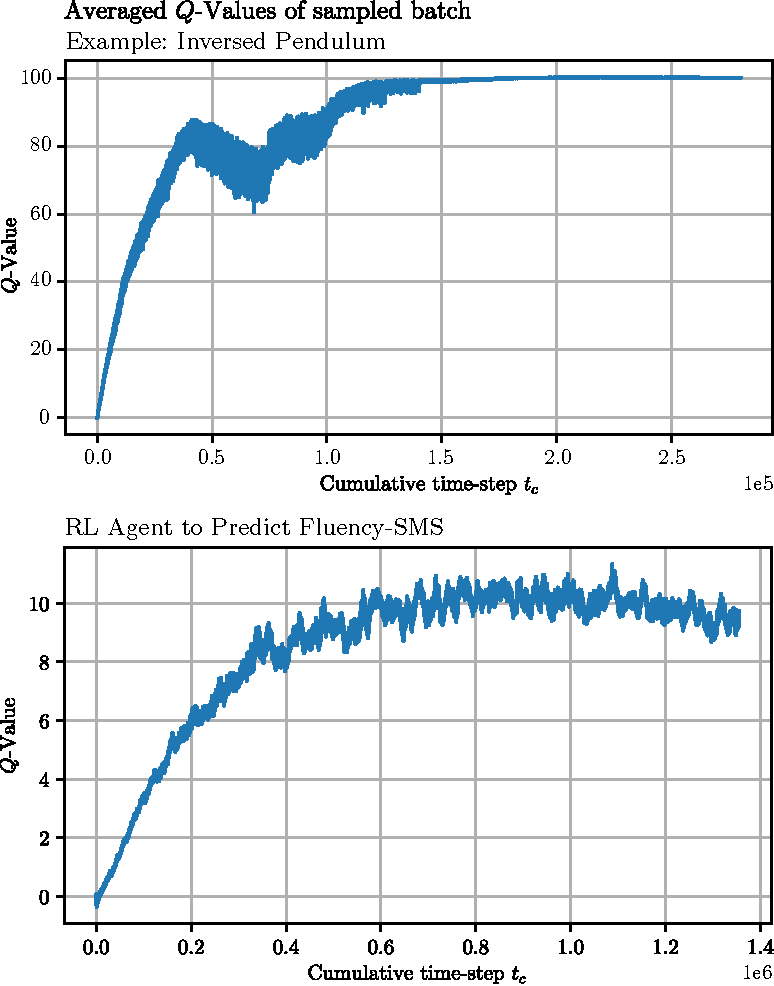
\includegraphics[width=0.75\textwidth]{QValuesFluency_and_Pendulum.pdf}
\caption{Averaged $Q$-Values per sampled batch at each training iteration for the example of balancing an inversed pendulum (top) and predicting the Fluency-SMS (bottom).} \label{fig:QValuesProgression}
\end{figure}

% %% Stride-Pair 1::
% %% Stride-Pair 2::
% Consider the following two stride-pairs, which will be referred to as SPI and SPII from the test dataset. SPI is a measured stride-pair of a critically affected patient (SMS of XX), and SPII, that of a mildly affected patient (SMS of XX). Both these handpicked examples have correctly predicted SMS, but not all predicted SMS subscores are necessarily correct. The true SMS subscores are displayed in brackets, next to the predicted subscores in Table \ref{tab:handpickedLTFMExamples} and as one can see, the selected key features vary depending on the physical status of a patient. The features listed in Table \ref{tab:handpickedLTFMExamples} are sorted in accordance to its relevance in terms of distinguishing samples of the selected stride-pair's assigned subscore from the remaining three subscores, quantified by the mutual information (cite??).

% \begin{table}[H]
%   \centering
%   \begin{tabular}{@{}l@{\hspace{0.25em}}|p{0.4\textwidth}p{0.4\textwidth}}
%     \hline
%     \textbf{Sub-} & \textbf{<Example A>} & \textbf{<Example B>} \\
%     \textbf{score} & $\quad$ \textbf{SMS: XX (critical)} & $\quad$ \textbf{SMS: XX (mild)} \\
%     \hline
%     \multirow{5}{*}{$\hspace{0.95em}$\makebox[0.75em]{\rotatebox{90}{\textbf{Trunk-SMS }}}}
%     & \textbf{Predicted score: XX} (XX) & \textbf{Predicted score: XX} (XX) \\ \cline{2-3}
%     & Feature A.2 & Feature B.2 \\
%     & Feature A.3 & Feature B.3 \\
%     & Feature A.4 & Feature B.4 \\
%     & $\cdots$ (XX features in total) & $\cdots$ (XX features in total) \\ \hline
%     \multirow{5}{*}{$\hspace{0.95em}$\makebox[0.75em]{\rotatebox{90}{\textbf{Leg-SMS }}}}
%     & \textbf{Predicted score: XX} (XX) & \textbf{Predicted score: XX} (XX) \\ \cline{2-3}
%     & Feature A.2 & Feature B.2 \\
%     & Feature A.3 & Feature B.3 \\
%     & Feature A.4 & Feature B.4 \\
%     & $\cdots$ (XX features in total) & $\cdots$ (XX features in total) \\ \hline
%     \multirow{5}{*}{$\hspace{0.95em}$\makebox[0.75em]{\rotatebox{90}{\textbf{Arm-SMS }}}}
%     & \textbf{Predicted score: XX} (XX) & \textbf{Predicted score: XX} (XX) \\ \cline{2-3}
%     & Feature A.2 & Feature B.2 \\
%     & Feature A.3 & Feature B.3 \\
%     & Feature A.4 & Feature B.4 \\
%     & $\cdots$ (XX features in total) & $\cdots$ (XX features in total) \\ \hline
%     \multirow{5}{*}{$\hspace{0.95em}$\makebox[0.75em]{\rotatebox{90}{\textbf{Speed-SMS }}}}
%     & \textbf{Predicted score: XX} (XX) & \textbf{Predicted score: XX} (XX) \\ \cline{2-3}
%     & Feature A.2 & Feature B.2 \\
%     & Feature A.3 & Feature B.3 \\
%     & Feature A.4 & Feature B.4 \\
%     & $\cdots$ (XX features in total) & $\cdots$ (XX features in total) \\ \hline
%     \multirow{5}{*}{$\hspace{0.95em}$\makebox[0.75em]{\rotatebox{90}{\textbf{Fluency-SMS }}}}
%     & \textbf{Predicted score: XX} (XX) & \textbf{Predicted score: XX} (XX) \\ \cline{2-3}
%     & Feature A.2 & Feature B.2 \\
%     & Feature A.3 & Feature B.3 \\
%     & Feature A.4 & Feature B.4 \\
%     & $\cdots$ (XX features in total) (XX) & $\cdots$ (XX features in total) (XX) \\ \hline
%     \multirow{5}{*}{$\hspace{0.95em}$\makebox[0.75em]{\rotatebox{90}{\textbf{Stability-SMS }}}}
%     & \textbf{Predicted score: XX} & \textbf{Predicted score: XX} \\ \cline{2-3}
%     & Feature A.2 & Feature B.2 \\
%     & Feature A.3 & Feature B.3 \\
%     & Feature A.4 & Feature B.4 \\
%     & $\cdots$ (XX features in total) & $\cdots$ (XX features in total) \\ \hline
%   \end{tabular}
%   \caption{Two examples from the test dataset, each with their respective subset of features recruited by the agent to predict each SMS subscores}
%   \label{tab:handpickedLTFMExamples}
% \end{table}
